\documentclass{article}

\usepackage[papersize={8.27in,11.69in},hmargin=0.5in,tmargin=1.055in,bmargin=1.055in,includehead]{geometry}
% paper size if 6in x 9in which is standard international size
% margin from top is 0.7in including header
% margin from bottom is 0.6in including footer
% book of two sided pages is specified, with horizontal margin of 0.6in
% binding offset is an additional 0.1in from centre fold.
% REAL textwidth is therefore 6 - 2*0.6 -0.1 = 4.7in = 11.938cm, 0.45\textwidth = 5.3721 cm with 3 margins of 0.3979cm
\usepackage{multicol}
\setlength{\columnsep}{0.27in}
%
\usepackage[
    %backend=bibtex,
    backend=biber,
    natbib=true,
    style=numeric,
    sorting=none,
    backref=true
]{biblatex} %,style=verbose-trad2
%\addbibresource{bib.bib}
\bibliography{bibliography}


\usepackage[explicit]{titlesec}
\usepackage{titletoc}
\usepackage{lmodern}
\usepackage{epigraph}
\usepackage{xpatch}  % All above used in titling
%
\usepackage{tikz}
%
\usepackage{pgfplots} % for better precision plots
\pgfplotsset{compat=1.10} % for newer version?
\usepgfplotslibrary{fillbetween} % for shading pgfplots

\usepackage{graphicx}
\usepackage{wrapfig} % for odd wrapping of text around figure
%
\usepackage{textcomp} % for currency %\usepackage[gen]{eurosym}
%
\usepackage{lipsum} %for filler text only
%
%\usepackage{bold-extra} % Used in Game Theory Section for bold sc's
\usepackage[T1]{fontenc}
%
\usepackage{mathtools}
\usepackage{amsthm}
\usepackage{bm} %for bold greeks
\usepackage{booktabs} %for better standard tables
\usepackage{longtable} %used for acronymns table
\usepackage{array} % for customising paragraph p columns alignment
\usepackage{tablefootnote} % obvious
\usepackage{arydshln} %for dotted v lines in tables
%
\usepackage{glossaries}
\usepackage{caption}
\usepackage{subcaption}
%
\usepackage{enumerate} %for lists
%
\usepackage{fancyhdr} %for custom page headers
%
\usepackage{imakeidx} % for indexing

%%% TIKZ Predefinitions
\usetikzlibrary{patterns}
\usetikzlibrary{decorations}
\tikzstyle{block} =
    [rectangle, draw
     % , fill=blue!20
      , text width=7.5em
      , text centered
      , node distance=3.5cm
      , rounded corners
      , minimum height=2em
      , scale =0.8]
\tikzstyle{blockL} =
    [rectangle, draw
     % , fill=blue!20
      , text width=7.5em
      , align=left
      , node distance=3.5cm
      , rounded corners
      , minimum height=2em
      , scale =0.8]
\tikzstyle{block20} =
    [rectangle, draw
     % , fill=blue!20
      , text width=9em
      , text centered
      , node distance=3.5cm
      , rounded corners
      , minimum height=2em
      , scale =0.8]
      \tikzstyle{block40} =
    [rectangle, draw
     % , fill=blue!20
      , text width=10.5em
      , text centered
      , node distance=3.5cm
      , rounded corners
      , minimum height=2em
      , scale =0.8]
 \tikzstyle{Vblock} =
    [rectangle, draw=none
     % , fill=blue!20
      , text width=15em
      , text centered
      , node distance=3.5cm
      , rounded corners
      , minimum height=2em
      , scale =0.8]
\tikzstyle{Lblock} =
    [rectangle, draw
     % , fill=blue!20
      , text width=35em
      , text centered
      , node distance=3.5cm
      , rounded corners
      , minimum height=2em
      , scale =0.8]
\tikzstyle{virtual} = [coordinate]
%%%%%%%%%%%%%%%%%%%%

\usepackage{sectsty}
\sectionfont{\centering}
\subsectionfont{\centering}
\usepackage{float} % for helping figures in twocol environ with [H]
\usepackage[font=small,labelfont=bf,textfont=it]{caption} % for caption text that
                                              % can be at all discerned
                                              % from normal text
 \newcommand{\fixme}[1]{{\color{red}#1}} 

\newenvironment{Figure}
  {\par\medskip\noindent\minipage{\linewidth}}
  {\endminipage\par\medskip}
\usepackage{lipsum}
\AtBeginDocument{\renewcommand{\bibname}{\centerline References}}

% Don't hyphenate UppSAT
\hyphenation{UppSAT}

%% {
	\centering
	\vspace{1cm}
	{\scshape\Huge\ UppSAT in the Cloud \par}
	\vspace{1cm}
	{\scshape\Large --- \par}
	\vspace{0.9cm}
	\begin{center}{Peter Backeman \& Albin Stjerna}\\
	Uppsala University, Uppsala, Sweden
	\end{center}
}

\title{\uppsat\ in the Cloud}
\author{Peter Backeman \& Albin Stjerna}

\begin{document}

\maketitle

\begin{multicols}{2}

\abstract{This paper describes a system for efficiently
      automating and scheduling a series of compute-heavy benchmarks, as
      exemplified by the SMT~solver {\uppsat}, using Docker containers on a
      virtualised Cloud platform based on OpenStack. It finds that switching to
      virtualised benchmarking immediately solves the $P=NP$ problem, cures
      cancer, and brings about world peace, in addition to providing an
      aesthetically perfect solution.}
  


\section*{Background}



The Satisfiability Modulo Theories (SMT) is the problem of solving
Boolean formulas where each propositional atom (in addition of being
either true or false) has an interpretation in some theory (e.g.,
linear arithmetic, bit-vectors). In many different areas, satisfying
assignments (solutions) for these kind of formulas are sought for, one
important use case being verification of hardware and software. For
example, in model checking, a SMT~formula is generated such that a
solution corresponds to a hardware or software bug. Therefore,
efficient SMT-solvers are highly desirable and there exists much
research in this field (see e.g.,~\cite{sathandbook} for an
introduction).

The satisfiability problem (solving Boolean formulas) is probably the
most famous NP-complete problem~\cite{satnp}, and SMT solvers must
additionaly use a decision procedure for the various background
theories, which results in a combination which is highly
complex. Therefore, prediciting the performance changes when trying
different strategies can be very hard, and usually extensive
benchmarking is used to evaluate new techniques.

These benchmarks are often run on local clusters or even local
machines in sequential order, leading to long waits from start until a
complete picture of the effects of the evaluated modifications are
yielded. By instead using a cloud approach, where not only the number
of machines could be scaled, but also dynamic load-balancing could be
used, this waiting time could be greatly reduced.

%% Maybe a reference to ``cloud approach'' above. But I am scared of picking a paper, since here they will actually now which papers are good :)

In this paper, we investigate how a SMT~solver can be adapted to allow
benchmarking in a cloud environment, with \uppsat~\cite{uppsat} as a
case study. The contribution of this paper are:

\begin{itemize}
  \item a partially automated testbed environment in the cloud with a
    complete continuous integration pipeline from code pushed to Git
    to it being benchmarked in the cloud.
    
  \item a Representational State Transfer (REST) API controlling the
    testbed environment
    
  \item a modular system of Docker containers~\cite{docker} which
    packages \uppsat for easy deployment

  \item an evaluation of how virtualisation affects measurement errors
    of benchmarks
\end{itemize}

We argue that the use of Docker serves the dual purpose of enhancing both
repeatability and traceability of the experiments, as the entire experiment
environment is packaged into containers, allowing the use of Docker's tools for
comparison and analysis of containers in the event of unexpected results.
Additionally, as an added benefit, Docker ensures clean separation of
experiments.


\section{\uppsat}
In this project we use the \uppsat SMT
solver \footnote{https://github.com/uuverifiers/uppsat} as a
benchmarking tool. It is an \emph{abstract} SMT solver -- it takes an
\emph{approximation} and a \emph{back-end} SMT solver as input and
yields an approximating SMT solver, illustrated in
Figure~\ref{fig:uppsat}. For a more comprehensive description,
see~\cite{uppsat}.

\begin{Figure}
\centering
\begin{tikzpicture}[node distance = 2cm] 
  \tikzstyle{level 1}=[sibling distance=45mm] 
  \tikzstyle{level 2}=[sibling distance=15mm] 
  \tikzstyle{level 3}=[sibling distance=8mm]
  \tikzstyle{rect} = [minimum width =2.5cm, minimum height=1cm]
  \tikzstyle{norm}=[edge from parent/.style={draw, thick}]

	\node[draw=none](aux){};
	\node[draw,rectangle,rect, dashed,below of=aux, align=center](approx){Approximations};
	\node[draw,rectangle,rect, below of=approx, below=-1cm, align=center](smt) {SMT};
	\node[draw=none, below of=smt](sat){SAT/UNSAT};
	\draw[->](aux.south)-- node[right=0.1cm, pos=.2](){$\phi$}(approx.north);
	\draw[->]([xshift=0.5cm]approx.south)--([xshift=0.5cm]smt.north);
	\draw[->]([xshift=-0.5cm]smt.north)--([xshift=-0.5cm]approx.south);
	\draw[->](smt.south)--(sat.north);
	\node[draw,inner sep=5mm,fit=(approx) (smt) ] {};	
\end{tikzpicture}
\label{fig:uppsat}
  \captionof{figure}{\uppsat\ composition}\label{fig:uppsat}
\end{Figure}

\subsection{Instances}
We will call the smallest kind of test an \emph{instance} and it consists of four parts:
\begin{itemize}
\item An approximation strategy
\item An \uppsat\ back-end
\item A timeout
\item A SMT problem (a benchmark)
\end{itemize}

We will not go into detail the different possible arguments here but
will quickly mention that in this study we will compare two
approximation strategies with about one hundred SMT problems, while
the back-end and timeout will remain fixed.

\section{\testbench}

Our system, \testbench, is an interactive batch processing system,
where experiments are submitted to a queue of jobs and then executed
by worker nodes. The system takes as input
\begin{itemize}
  \item A set of approximation strategies
  \item A set of \uppsat\ back-ends
  \item One timeout
  \item A set of SMT problems
\end{itemize}
\testbench then evaluates the cross product of all these configuration
and reports on the results. This corresponds to a complete testing of
all the presented parameters of the system.

\subsection*{REST API Design}

This functionality is represented as two REST endpoints \texttt{/experiment},
and \texttt{/experiment/<ID>}. A \texttt{POST}~request (illustrating
non-idempotency) to \texttt{/experiment} will start a new experiment, assigning
it a unique ID, and redirecting the user to \texttt{/experiment/<ID>}, where it
can be queried for its status (using a \texttt{GET}~request). Experiments can
then be canceled (if running) and deleted via the \texttt{DELETE}~request to
their endpoint.

\subsection*{System Design and Implementation}

The implementation is based on the Celery task queue~\cite{celery}, and packaged
in Docker~\cite{docker} containers. The front-end REST API receives input from
the user, unpacks the experiment into a set of trials, and submits them to the
Celery task queue (via RabbitMQ) for processing. Each worker, with identical
configuration, listens on the task queue, fetches tasks, and executes them,
storing the results back into Celery (via Redis). The user can then, via the
front-end REST API, query experiments for progress as they are executing, and is
also able to cancel tasks via the \texttt{DELETE} command. An illustration of
the architecture can be seen in Figure~\ref{fig:architecture}.

\begin{Figure}
  \centering
  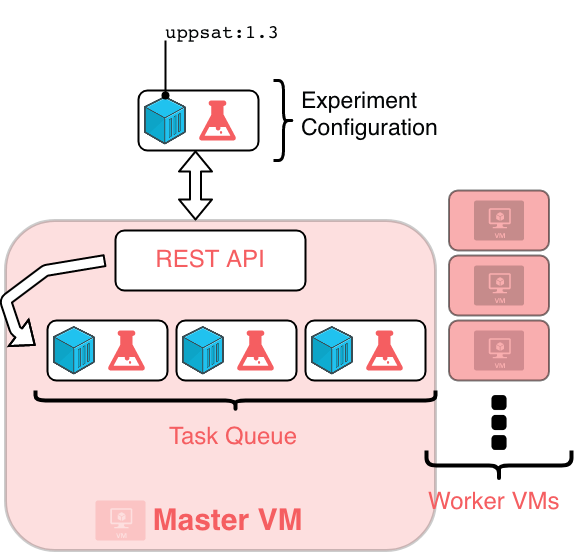
\includegraphics[width=0.9\textwidth]{architecture}
  \captionof{figure}{An overview of the architecture of \testbench.}\label{fig:architecture}
\end{Figure}

As experiments are executed inside of Docker containers, the host machine's
control socket is bind-mounted into the Docker container running the workers,
such that the worker effectively spawns and runs experiments at the same
containment level as itself. The runtime reported is the runtime seen by Docker.

\subsection*{Cloud Environment and Provisioning}

\testbench is configured in a OpenStack cloud environment~\cite{openstack}, using
HEAT orchestration templates for provisioning. The base VMs are running
Ubuntu~\fixme{18.08}. RabbitMQ, Redis, and the front-end API are all installed
on a (\texttt{small}) separate VM (called the master) in order to avoid interference
with the experiments. Each worker VM (\texttt{medium}) receives the same
configuration; a clean installation of the Docker community edition, the address
of the master VM, and a Docker container mounting a shared folder via NFS from
the master for sharing benchmark files. All workers immediately start up a
container running a worker instance upon booting and finishing provisioning.
These worker instances were intentionally configured to only execute one task at
a time, for optimal isolation between trials.

It is worth mentioning that \testbench is designed to be relatively independent
of the underlying architecture. Therefore, it can easily be executed on ``bare
metal'' hardware as well as on virtual machines.

\section*{Results}
Both as a demonstration of the usability of the system as well as
evaluating measurement errors due to virtualization a number of tests
were executed on \testbench. We used the following parameters:
\begin{itemize}
\item Two approximation strategies are used, \emph{Reduced Point
  Floating Point}, presented in \cite{uppsat}, and \emph{bit-vector
  approximation}, presented in \cite{joel}.

\item One back-end is used, namely \emph{z3}\footnote{https://github.com/Z3Prover/z3}  .

\item A fixed timeout of 60 seconds is used.

\item A set of 130 benchmarks is used, consisting of satisfiable
  instances of the quantifier free floating point segment of the
  SMT-LIB\cite{smtlib}.
\end{itemize}

%% Fix Joel citation


\subsection*{Measurement Errors in Our Cloud Environment}
\fixme{In which we report on the standard deviation and therefore the
  reliability of our experiments when run on virtualised hardware and ideally
  find that it's as close to zero as possible.}

\subsection*{Benchmark Lead Time Comparison}
 \fixme{Here we do some comparison on how long it takes to finish a set of benchmarks,
   compared to going by the manual approach, ideally finding that it's as close
   to positive infinity as possible.}


\section*{Discussion}

\fixme{\lipsum[66]}

\section*{Conclusion}

\fixme{\lipsum[100]}

\printbibliography

\end{multicols}
\end{document}
